\documentclass{beamer}

\usepackage[utf8]{inputenc}%           gestion des accents (source)
\usepackage[T1]{fontenc}%              gestion des accents (PDF)
\usepackage[francais]{babel}%          gestion du français
\usepackage{textcomp}%                 caractères additionnels
\usepackage{mathtools,  amssymb, amsthm}% packages de l'AMS + mathtools
\usepackage{lmodern}%                  police de caractère
\usepackage{geometry}%                 gestion des marges
\usepackage{graphicx}%                 gestion des images
\usepackage{xcolor}%                   gestion des couleurs
\usepackage{array}%                    gestion améliorée des tableaux
\usepackage{calc}%                     syntaxe naturelle pour les calculs
\usepackage[framemethod=TikZ]{mdframed}% print frames
\usepackage[justification=centering]{caption}%                  for captionof
\usepackage{listings}%				  pour insertion de codes 
\usepackage{enumitem}%                 pour les listes numérotées
\usepackage{microtype}%                améliorations typographiques
\usepackage{csvsimple}%                convertir un fichier .csv en tableau
\usepackage{url}%					  amélioration afficahge url
\usepackage{hyperref}%                 gestion des hyperliens
\usepackage{svg}	%					  gestion des svg	
\usepackage{float}%					  gestion des figure non flotante
 
\lstset{language=c++}
\definecolor{codegreen}{rgb}{0,0.6,0}
\definecolor{codegray}{rgb}{0.5,0.5,0.5}
\definecolor{codepurple}{rgb}{0.58,0,0.82}
\definecolor{backcolour}{rgb}{0.95,0.95,0.92}
 
\lstdefinestyle{mystyle}{
    backgroundcolor=\color{backcolour},   
    commentstyle=\color{codegreen},
    keywordstyle=\color{magenta},
    numberstyle=\tiny\color{codegray},
    stringstyle=\color{codepurple},
    basicstyle=\footnotesize,
    breakatwhitespace=false,         
    breaklines=true,                 
    captionpos=b,                    
    keepspaces=true,                 
    numbers=left,                    
    numbersep=5pt,
    otherkeywords={uint16_t},                  
    showspaces=false,                
    showstringspaces=false,
    inputencoding=latin1,
    showtabs=false,                  
    tabsize=2
}
\lstset{style=mystyle}

\hypersetup{%
    pdfborder = {0 0 0}
}

\usetheme{Warsaw}

\setbeamersize{text margin left=15px}
\setbeamersize{text margin right=15px}


\title{Rapport du Projet PSAR}
\subtitle{Dispositif Autonome de Synthèse Sonore}
\institute{Encadrant : Hugues Genevois}
\author{Pierre Mahé}
\date{\today}

\titlegraphic{
	
\includegraphics[height=20px]{upmc_logo.jpg}	
	\hspace{4cm}
	
\includegraphics[height=20px]{LogoLAM.jpg}}
\begin{document}

\begin{frame}
\titlepage
\end{frame}


\begin{frame}
\frametitle{Contrainte du projet}
\framesubtitle{La Carte Udoo}
\begin{minipage}{0.49\textwidth}
\textbf{Avantage:}
\begin{itemize}
\item Compatibilité Arduino
\item Bonne plate-forme d’expérimentation
\item Distribution Linux
\item Prix raisonnable
\end{itemize}
\end{minipage}
\begin{minipage}{0.49\textwidth}
\begin{figure}
  \centering
  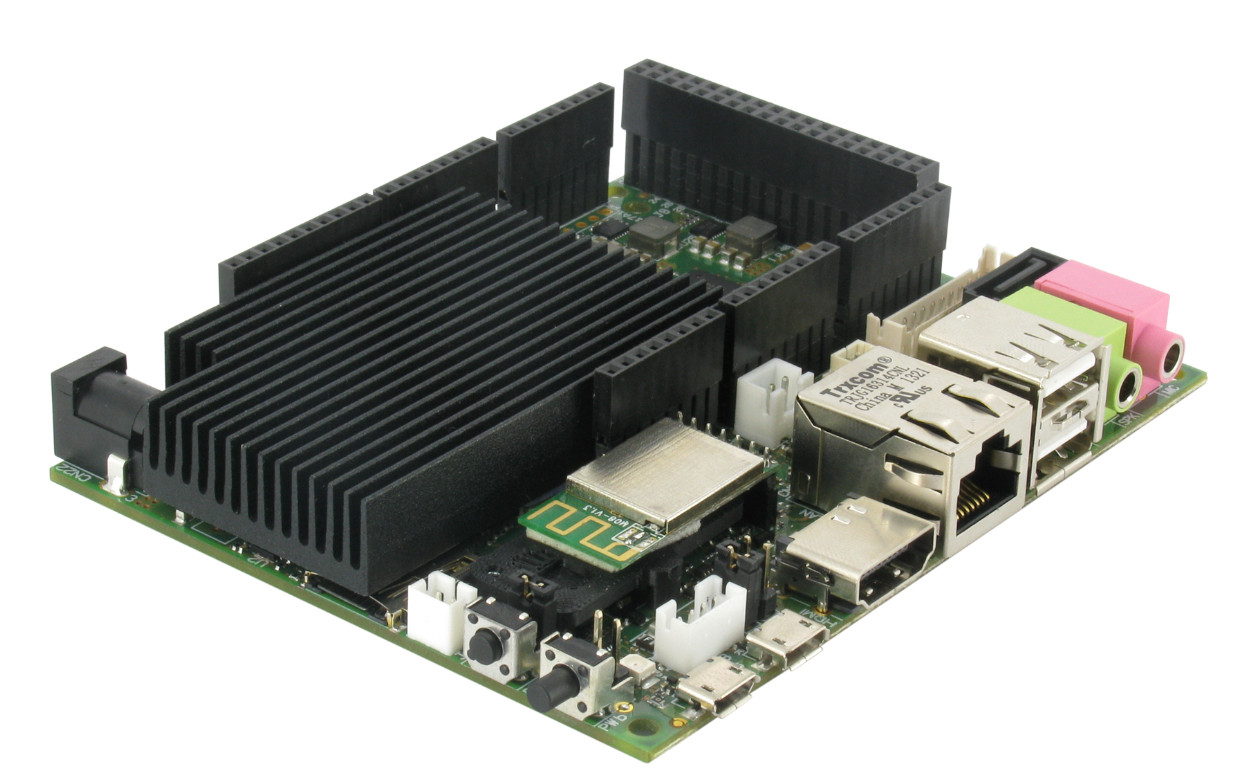
\includegraphics[width=\textwidth]{udoo.jpg} 
	\caption{Carte Udoo}
\end{figure}
\end{minipage}
\end{frame}


\begin{frame}
\frametitle{Contrainte du projet}
\framesubtitle{Pure Data}
\textbf{Pure Data}
\begin{itemize}
\item Langage Graphique pour la création et l'interaction musical temps réel.
\item Possibilité de définir des nouveaux modules appelés boites.
\item Possibilité de créer des modules appelé \texttt{External} grâce à \texttt{Flext}.
\item Possibilité de modifier les patchs durant l’exécution du programme.
\item Il existe une grande communauté d'utilisateurs, de nombreuse fonctionnalité sont déjà implémenté.
\end{itemize}
\end{frame}

\begin{frame}
\frametitle{Contrainte du projet}
\framesubtitle{Pure Data}
\textbf{Exemple de Patch}
\begin{figure}
  \centering
  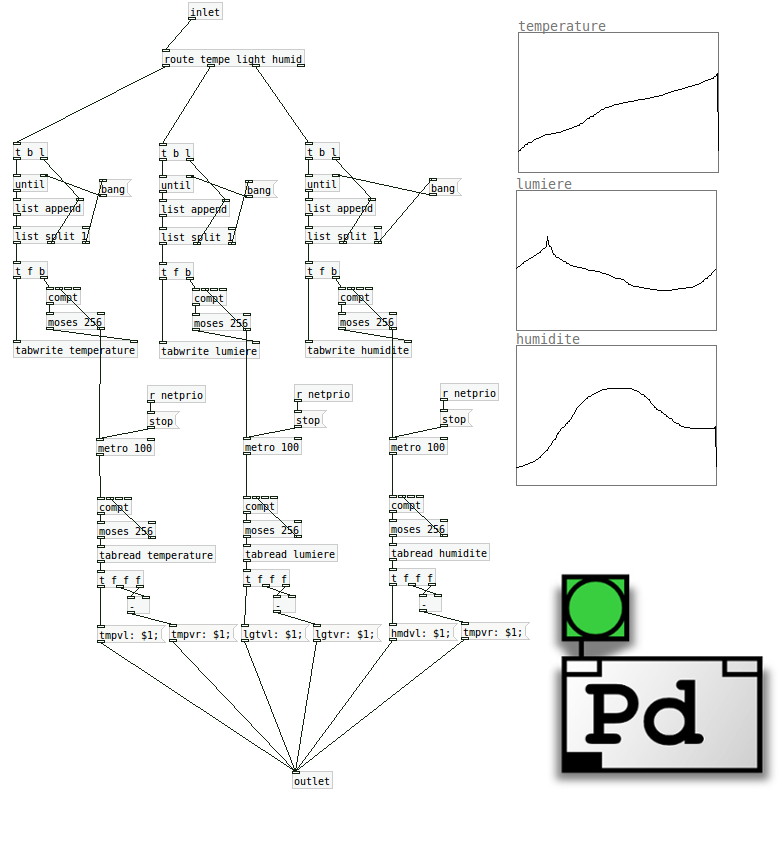
\includegraphics[width=160px]{pd.jpg} 
	\caption{Patch Pd}
\end{figure}

\end{frame}


\begin{frame}
\frametitle{Structure du projet}
\begin{figure}
  \centering
  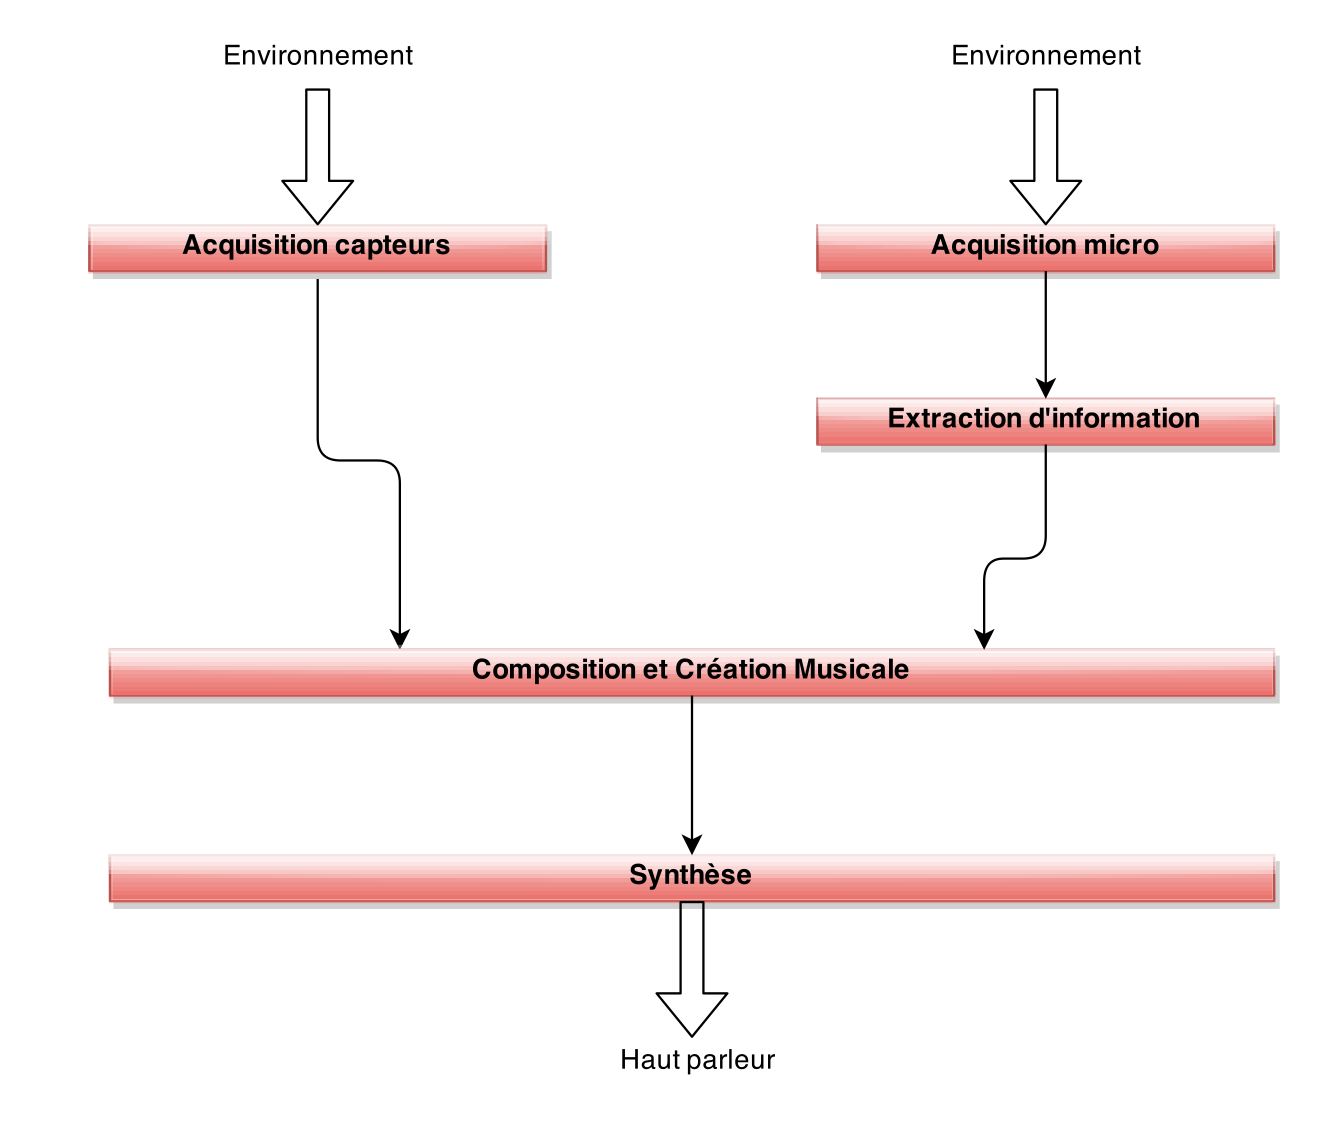
\includegraphics[height=220px]{structprojet.jpg} 
\end{figure}
\end{frame}


\begin{frame}
\frametitle{Récupération de l'environnement}
\begin{figure}
  \centering
  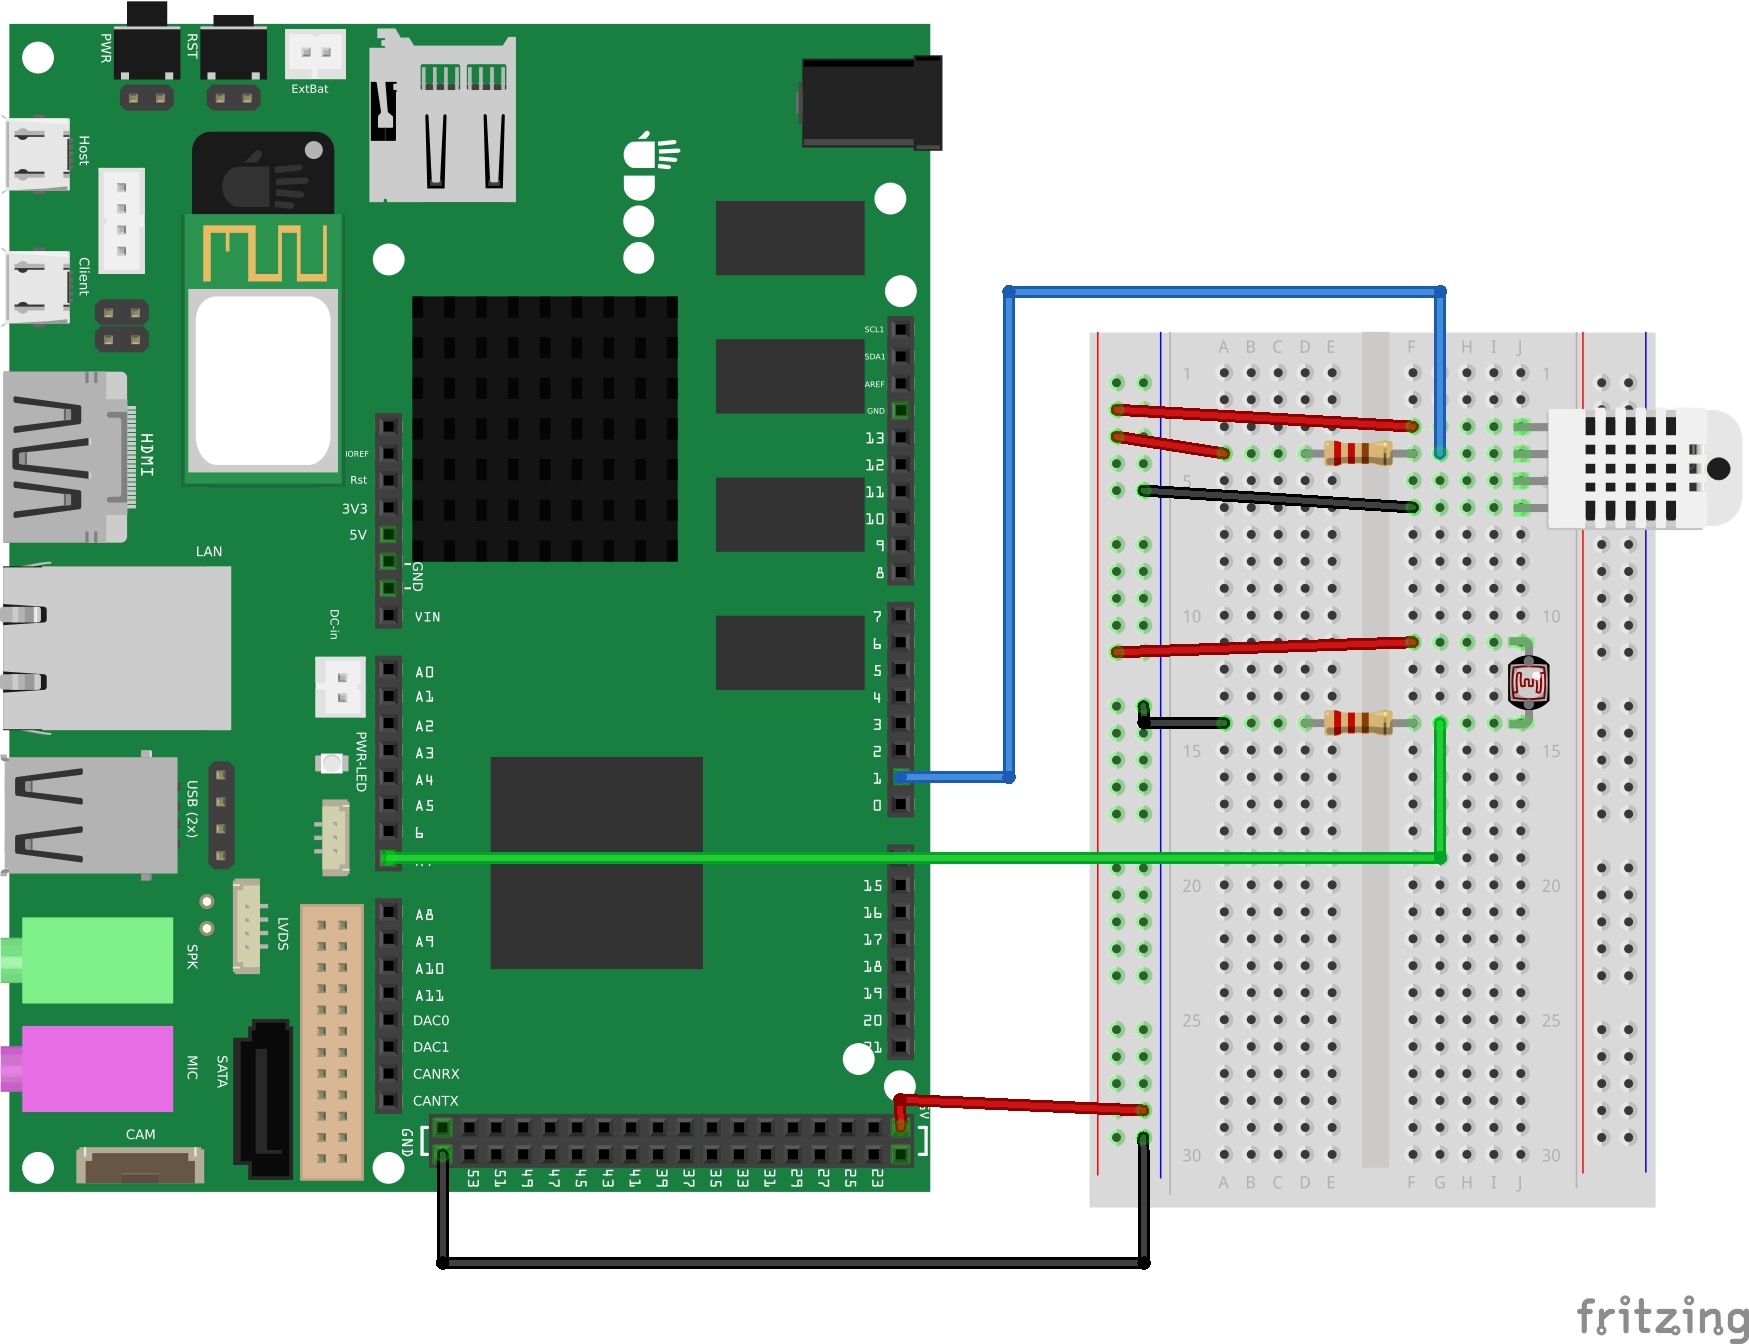
\includegraphics[width=150px]{montage.jpg}  
  \hspace{15px}
  \includegraphics[width=150px]{montagephoto.jpg} 
	\caption{Montage sur la carte Udoo}
\end{figure}
\end{frame}

\begin{frame}
\frametitle{Récupération de l'environnement}

\textbf{Communication inter plate-forme}
\begin{figure}
\centering
\includegraphics[height=30px]{protocole.jpg}
\end{figure}
\textbf{External pour la communication}
\begin{figure}
\centering
\includegraphics[height=120px]{protocole2.jpg}
\end{figure}
\end{frame}

\begin{frame}
\frametitle{Traitement audio}
\framesubtitle{Traitement bas niveau - première approche}
De prime abord, la Transformée de Fourier apparaissait comme la meilleur solution.\\
La carte ayant des ressources limité, la solution fut abandonnée au profit d'une technique plus économe en ressources.

\begin{figure}
\centering
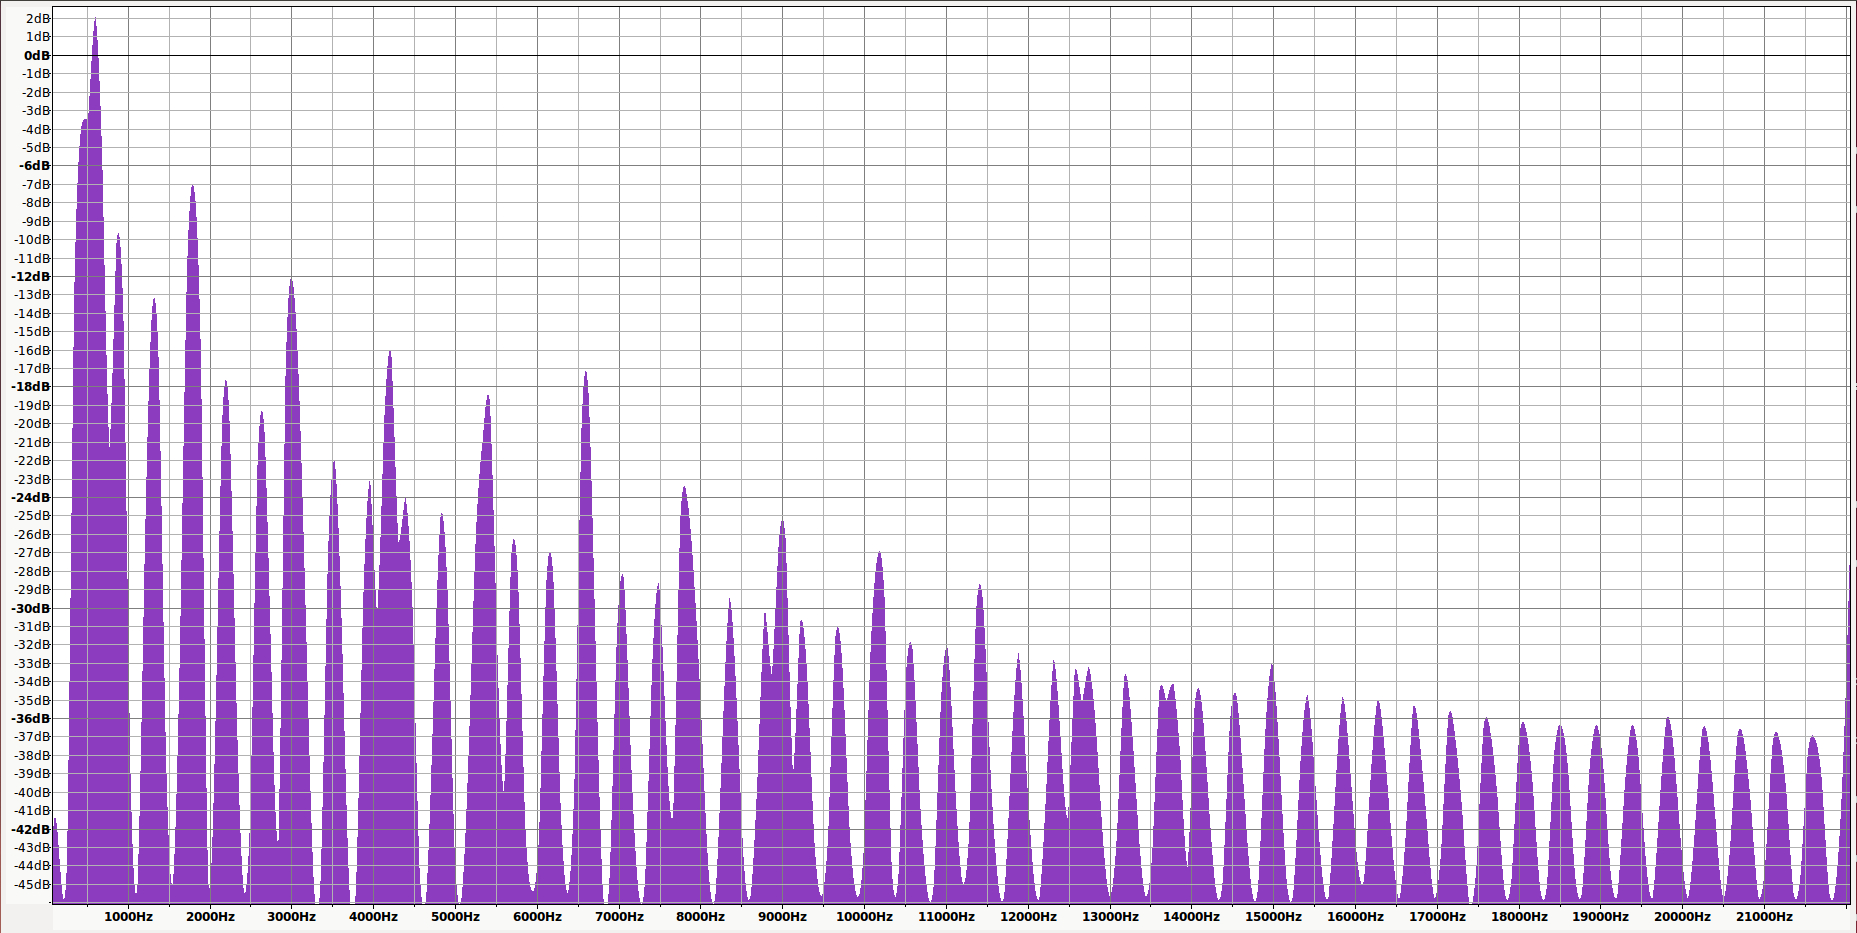
\includegraphics[height=100px]{fft.jpg}
\caption{Transformée de Fourier}
\end{figure}
\end{frame}


\begin{frame}
\frametitle{Traitement audio}
\framesubtitle{Traitement bas niveau - seconde approche}

Partage du spectre sonore en plusieurs bandes de fréquences à l'aide de filtres puis de détecter la fréquence principale de chaque bande.
\begin{figure}
\centering
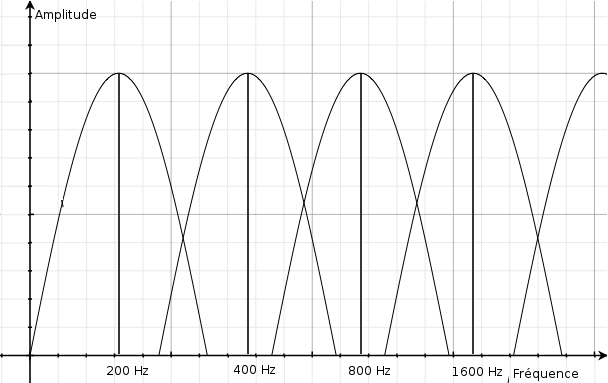
\includegraphics[height=100px]{filtre.jpg}
\caption{Filtrage par bandes}
\end{figure}
Les filtres sont espacés d'une octave.\\
Pour limiter les fausses détections, à la sortie de chaque filtre des \texttt{Nose Gates} ont été ajoutés. 
\end{frame}


\begin{frame}
\frametitle{Traitement audio}
\framesubtitle{Traitement bas niveau - autres traitements}
\textbf{Détecteur de notes}\\
Un compteur de notes fourni périodiquement la fréquence d'apparition de chaque note.
\\ 
\textbf{Bande de fréquences}\\
Pour ne pas perdre l'information sur la hauteur du son capté par le micro.\\
Le dispositif conserve aussi la répartition des fréquences.

\end{frame}


\begin{frame}
\frametitle{Traitement audio}
\framesubtitle{Traitement haut niveau - Mélodie et Rythme}
Une information importante en plus de la Mélodie et le rythme, pour jouer des sons cohéritant avec l’environnement.\\
Création d'un module pour détecter le début de notes à l'aide de la boite \texttt{bonk} qui détecte les impacts dans un signal.

\begin{figure}
\centering
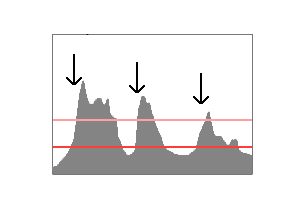
\includegraphics[height=130px]{bonk.jpg}
\caption{Fonctionnement de \texttt{bonk}}
\end{figure}
\end{frame}


\begin{frame}
\frametitle{Traitement audio}
\framesubtitle{Traitement haut niveau - Détection de Motif minimal}
Groupement des rythmes détecté en sequence.\\
Le module procède à une normalisation de la duré des rythmes.
\begin{figure}
\centering
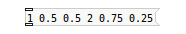
\includegraphics[height=20px]{rythme.jpg}
\caption{Séquence rythmique détecté}
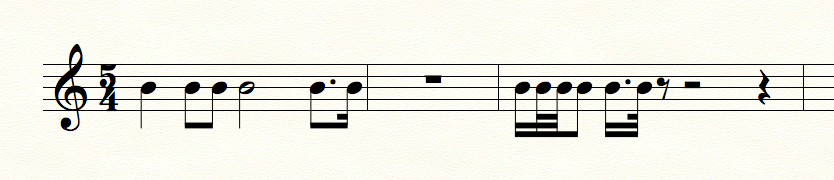
\includegraphics[height=50px]{structurerythme.jpg}
\caption{Séquence rythmique pouvant produire la séquence}
\end{figure}
\end{frame}

\begin{frame}
\frametitle{Traitement audio}
\framesubtitle{Traitement haut niveau - Détection de Motif minimal}
Pour plus d'interactivité, le dispositif retourne le premier motif rythmique trouvé, et non le motif rythmique le plus long.\\
La taille du motif est paramétrable.
\begin{figure}
\centering
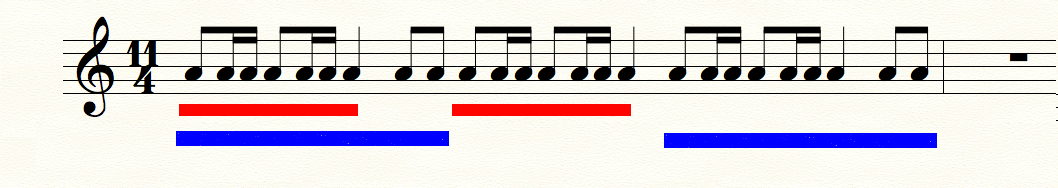
\includegraphics[height=50px]{motifrythme.jpg}
\caption{Motif rythmique}
\end{figure}
\end{frame}


\begin{frame}
\frametitle{Interface Utilisateur}
\begin{minipage}{0.49\textwidth}
\textbf{Permet à l'utilisateur}\\\\
L'envoi de données pour simuler les données collectés par les capteurs.\\\\
Changement du module de Création Musicale
\end{minipage}
\begin{minipage}{0.49\textwidth}
\begin{figure}
  \centering
  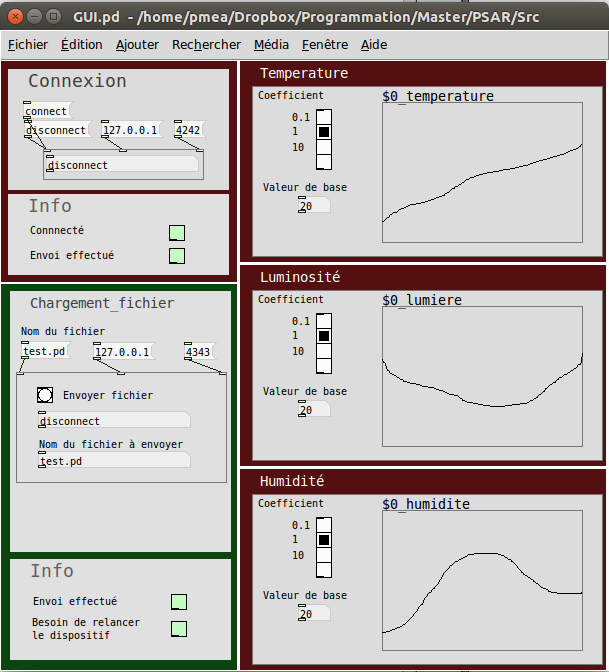
\includegraphics[width=\textwidth]{GUI.jpg} 
	\caption{Interface utilisateur}
\end{figure}
\end{minipage}
\end{frame}


\begin{frame}
\frametitle{Pour aller plus loin}
\framesubtitle{Les Tests}
\textbf{Tests en environnement réel}\\
Les sons de l'environnement étant de nature très diverses, il est difficile de pouvoir tous les cas possibles.\\
Des testes supplémentaires en environnement réel auraient était pertinents.
\newline
\newline
\textbf{Tests énergétique}\\
La carte Udoo étant tres énergivore, il serait intéressant de tester le dispositif sur d'autre carte moins gourmande en énergie.
\newline
\newline
\textbf{Serveur distant}\\
Dans l'optique d'econnomie d'energie, il serait intéressant de réflechir à un version avec un serveur, où le traitement des capteurs serait fait sur celui ci.
\end{frame}
\end{document}